%%%%%%%%%%%%%%%%%%%%%%%%%%%%%%%%%%%%%%%%%%%%%%%%%%%%%%%%%%%%%%%%%%%%%%%%
%                                                                      %
%     File: Introduction/03_SystemOverview.tex                         %
%     Tex Master: ../Thesis.tex                                        %
%                                                                      %
%%%%%%%%%%%%%%%%%%%%%%%%%%%%%%%%%%%%%%%%%%%%%%%%%%%%%%%%%%%%%%%%%%%%%%%%

% ==============================================================================
\section{Proposed Approach}
\label{sec:intro_system_overview}

% How are the two vehicles coordinated?
Each vehicle is controlled by its own \gls{nmpc}, which predicts the motion of the vehicle with a model derived from its physics, and plans it within the limits of the vehicle over a horizon and a sampling time suited to its dynamics. The two controllers exchange the trajectories they predict, so that each keeps the separation within the reach of the tether by taking into account where the other vehicle is going, rather than where it is.

% How is the tether taken into account?
The controller of the \gls{uav} also predicts the force that the hanging tether applies on it, with a model that accounts for its weight. This model assumes that the slack of the tether is kept constant by a winch on the deck of the \gls{usv}, which spools the tether in and out as the distance between the vehicles changes. The forces that the models do not describe, such as the wind, are compensated by a disturbance observer, which estimates them from the motion of the \gls{uav}.

% And how do the controllers know where to go?
The controllers follow references, but do not decide where each vehicle should go. This is the role of the manoeuvres, such as a takeoff, a formation or a landing, which give the reference of each vehicle at every instant, and of the missions, which chain the manoeuvres of both vehicles into a complete operation. Since the controllers keep the vehicles within their limits whatever reference they are given, the manoeuvres can remain simple. An operator selects and launches the missions from a web interface, the Mission Control Centre. Figure~\ref{fig:intro_system_overview} shows how these parts fit together.

\begin{figure}[htbp]
    \centering
    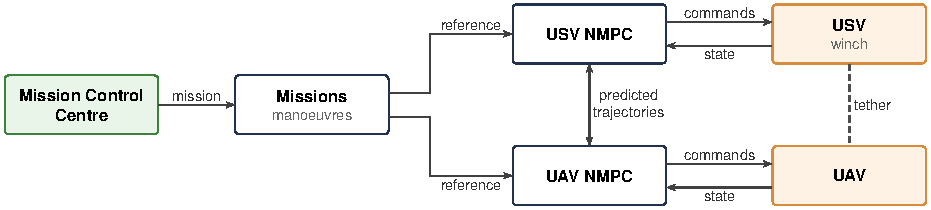
\includegraphics[width=\linewidth]{Introduction/figures/system_overview.pdf}
    \caption{Overview of the proposed system.}
    \label{fig:intro_system_overview}
\end{figure}
